% Options for packages loaded elsewhere
\PassOptionsToPackage{unicode}{hyperref}
\PassOptionsToPackage{hyphens}{url}
%
\documentclass[
]{book}
\usepackage{amsmath,amssymb}
\usepackage{lmodern}
\usepackage{iftex}
\ifPDFTeX
  \usepackage[T1]{fontenc}
  \usepackage[utf8]{inputenc}
  \usepackage{textcomp} % provide euro and other symbols
\else % if luatex or xetex
  \usepackage{unicode-math}
  \defaultfontfeatures{Scale=MatchLowercase}
  \defaultfontfeatures[\rmfamily]{Ligatures=TeX,Scale=1}
\fi
% Use upquote if available, for straight quotes in verbatim environments
\IfFileExists{upquote.sty}{\usepackage{upquote}}{}
\IfFileExists{microtype.sty}{% use microtype if available
  \usepackage[]{microtype}
  \UseMicrotypeSet[protrusion]{basicmath} % disable protrusion for tt fonts
}{}
\makeatletter
\@ifundefined{KOMAClassName}{% if non-KOMA class
  \IfFileExists{parskip.sty}{%
    \usepackage{parskip}
  }{% else
    \setlength{\parindent}{0pt}
    \setlength{\parskip}{6pt plus 2pt minus 1pt}}
}{% if KOMA class
  \KOMAoptions{parskip=half}}
\makeatother
\usepackage{xcolor}
\IfFileExists{xurl.sty}{\usepackage{xurl}}{} % add URL line breaks if available
\IfFileExists{bookmark.sty}{\usepackage{bookmark}}{\usepackage{hyperref}}
\hypersetup{
  pdftitle={The Medieval Islamicate World: 570-1250 تاريخ الإسلام/תאריֹךֹ אלאסאם},
  pdfauthor={Lecturer: Aslisho Qurboniev},
  hidelinks,
  pdfcreator={LaTeX via pandoc}}
\urlstyle{same} % disable monospaced font for URLs
\usepackage{color}
\usepackage{fancyvrb}
\newcommand{\VerbBar}{|}
\newcommand{\VERB}{\Verb[commandchars=\\\{\}]}
\DefineVerbatimEnvironment{Highlighting}{Verbatim}{commandchars=\\\{\}}
% Add ',fontsize=\small' for more characters per line
\usepackage{framed}
\definecolor{shadecolor}{RGB}{248,248,248}
\newenvironment{Shaded}{\begin{snugshade}}{\end{snugshade}}
\newcommand{\AlertTok}[1]{\textcolor[rgb]{0.94,0.16,0.16}{#1}}
\newcommand{\AnnotationTok}[1]{\textcolor[rgb]{0.56,0.35,0.01}{\textbf{\textit{#1}}}}
\newcommand{\AttributeTok}[1]{\textcolor[rgb]{0.77,0.63,0.00}{#1}}
\newcommand{\BaseNTok}[1]{\textcolor[rgb]{0.00,0.00,0.81}{#1}}
\newcommand{\BuiltInTok}[1]{#1}
\newcommand{\CharTok}[1]{\textcolor[rgb]{0.31,0.60,0.02}{#1}}
\newcommand{\CommentTok}[1]{\textcolor[rgb]{0.56,0.35,0.01}{\textit{#1}}}
\newcommand{\CommentVarTok}[1]{\textcolor[rgb]{0.56,0.35,0.01}{\textbf{\textit{#1}}}}
\newcommand{\ConstantTok}[1]{\textcolor[rgb]{0.00,0.00,0.00}{#1}}
\newcommand{\ControlFlowTok}[1]{\textcolor[rgb]{0.13,0.29,0.53}{\textbf{#1}}}
\newcommand{\DataTypeTok}[1]{\textcolor[rgb]{0.13,0.29,0.53}{#1}}
\newcommand{\DecValTok}[1]{\textcolor[rgb]{0.00,0.00,0.81}{#1}}
\newcommand{\DocumentationTok}[1]{\textcolor[rgb]{0.56,0.35,0.01}{\textbf{\textit{#1}}}}
\newcommand{\ErrorTok}[1]{\textcolor[rgb]{0.64,0.00,0.00}{\textbf{#1}}}
\newcommand{\ExtensionTok}[1]{#1}
\newcommand{\FloatTok}[1]{\textcolor[rgb]{0.00,0.00,0.81}{#1}}
\newcommand{\FunctionTok}[1]{\textcolor[rgb]{0.00,0.00,0.00}{#1}}
\newcommand{\ImportTok}[1]{#1}
\newcommand{\InformationTok}[1]{\textcolor[rgb]{0.56,0.35,0.01}{\textbf{\textit{#1}}}}
\newcommand{\KeywordTok}[1]{\textcolor[rgb]{0.13,0.29,0.53}{\textbf{#1}}}
\newcommand{\NormalTok}[1]{#1}
\newcommand{\OperatorTok}[1]{\textcolor[rgb]{0.81,0.36,0.00}{\textbf{#1}}}
\newcommand{\OtherTok}[1]{\textcolor[rgb]{0.56,0.35,0.01}{#1}}
\newcommand{\PreprocessorTok}[1]{\textcolor[rgb]{0.56,0.35,0.01}{\textit{#1}}}
\newcommand{\RegionMarkerTok}[1]{#1}
\newcommand{\SpecialCharTok}[1]{\textcolor[rgb]{0.00,0.00,0.00}{#1}}
\newcommand{\SpecialStringTok}[1]{\textcolor[rgb]{0.31,0.60,0.02}{#1}}
\newcommand{\StringTok}[1]{\textcolor[rgb]{0.31,0.60,0.02}{#1}}
\newcommand{\VariableTok}[1]{\textcolor[rgb]{0.00,0.00,0.00}{#1}}
\newcommand{\VerbatimStringTok}[1]{\textcolor[rgb]{0.31,0.60,0.02}{#1}}
\newcommand{\WarningTok}[1]{\textcolor[rgb]{0.56,0.35,0.01}{\textbf{\textit{#1}}}}
\usepackage{longtable,booktabs,array}
\usepackage{calc} % for calculating minipage widths
% Correct order of tables after \paragraph or \subparagraph
\usepackage{etoolbox}
\makeatletter
\patchcmd\longtable{\par}{\if@noskipsec\mbox{}\fi\par}{}{}
\makeatother
% Allow footnotes in longtable head/foot
\IfFileExists{footnotehyper.sty}{\usepackage{footnotehyper}}{\usepackage{footnote}}
\makesavenoteenv{longtable}
\usepackage{graphicx}
\makeatletter
\def\maxwidth{\ifdim\Gin@nat@width>\linewidth\linewidth\else\Gin@nat@width\fi}
\def\maxheight{\ifdim\Gin@nat@height>\textheight\textheight\else\Gin@nat@height\fi}
\makeatother
% Scale images if necessary, so that they will not overflow the page
% margins by default, and it is still possible to overwrite the defaults
% using explicit options in \includegraphics[width, height, ...]{}
\setkeys{Gin}{width=\maxwidth,height=\maxheight,keepaspectratio}
% Set default figure placement to htbp
\makeatletter
\def\fps@figure{htbp}
\makeatother
\setlength{\emergencystretch}{3em} % prevent overfull lines
\providecommand{\tightlist}{%
  \setlength{\itemsep}{0pt}\setlength{\parskip}{0pt}}
\setcounter{secnumdepth}{5}
\usepackage{booktabs}
\ifLuaTeX
  \usepackage{selnolig}  % disable illegal ligatures
\fi
\usepackage[]{natbib}
\bibliographystyle{plainnat}

\title{The Medieval Islamicate World: 570-1250 تاريخ الإسلام/תאריֹךֹ אלאסאם}
\author{Lecturer: Aslisho Qurboniev}
\date{2022-05-02}

\begin{document}
\maketitle

{
\setcounter{tocdepth}{1}
\tableofcontents
}
\hypertarget{course-description}{%
\chapter{Course description}\label{course-description}}

The aim of this course is to provide an introduction to the early and medieval history of the Islamic world, from the rise of Islam in Arabia to the formation of a world civilisation. Students will learn how to relate ideas to historical, geographical, and material factors. Particular attention will be paid to religious and cultural continuity, as a backdrop to the evolution of an Islamic identity and institutions of government, administration, and education.

\hypertarget{intended-learning-outcomes}{%
\section{Intended learning outcomes}\label{intended-learning-outcomes}}

\begin{enumerate}
\def\labelenumi{\arabic{enumi}.}
\tightlist
\item
  Students will learn about the most important developments in Islamic history, main questions in the historiography of Islam, and be able to reflect historically and critically about a range of topics related to the way Muslim societies functioned in the past.
\item
  They will be able to find their way around major reference works for Islamic history and gain some familiarity with some primary sources.
\item
  They will learn how to write critical essays following the conventions of style and referencing in the field of Islamic history.
\item
  They will be able to apply the skills and methodological approaches to other subjects of study. They will be able to situate topics from Islamic studies in their historical context.
\item
  They will gain exposure to innovative approaches to the study of medieval Islamicate history, digital methods and techniques, and will be able to use apply skills in other areas of their interests.
\end{enumerate}

\hypertarget{lectures}{%
\section{Lectures}\label{lectures}}

Weekly lectures will cover the period from the rise of Islam in Late Antiquity to the decline of the major caliphates and the appearances of new polities ruled mostly by non-Arabs, culminating with the Mongol invasion of the Middle East by the end of the 1250s CE. Each lecture will highlight historiographical issues, which will then be picked up during the seminars.

\hypertarget{seminars}{%
\section{Seminars}\label{seminars}}

Seminars will follow the themes of the lectures but will expect input from students. For this, in addition to the discussion of secondary sources, students will be expected to engage with short excerpts from primary sources listed in the syllabus. Presentations will also take place during the seminars.

To prepare for the seminars you must read the weekly readings listed first closely as these will provide you with the general framework. Reading these will help you to be more selective about books and articles recommended for further reading. The short primary source readings are also essential for the seminars. All of this will help you with the exams.

\hypertarget{assessment}{%
\section{Assessment}\label{assessment}}

**Essay (50\%), open-book exam (30\%), presentation (15\%), participation (5\%).

\textbf{\emph{Essay,}} of maximum 2500 words. Essay questions will be drawn from the lectures and seminars topics and will be given one week before the submission date. You will be expected to be able to connect several topics and draw upon readings from several weeks, in addition to topic specific readings which will be provided with the questions.

\textbf{\emph{Open-book exam.}} The questions for open-book exam will be based on the list of books provided in the end of this syllabus. You will be asked to answer one of the questions within three hours, drawing on your knowledge of the course materials. The response must demonstrate a good overall understanding of the topics of Islamic history, an ability to select relevant material, and a close engagement with the selected books that you will have access to during the exam. You will not be penalised for poor referencing, spelling mistakes, and typos.

\textbf{\emph{Presentation.}} You will choose to present on one of the weekly topics, during one of the seminars. A strong presentation will combine a good understanding of the readings and an engaging and convincing use of material and archaeological evidence.

\textbf{\emph{Participation.}} It is essential to attend the lectures and seminars. You will be marked on your contributions to class discussions.

\hypertarget{resources-and-reading-materials}{%
\section{Resources and reading materials}\label{resources-and-reading-materials}}

\hypertarget{reference-works}{%
\subsection{Reference Works}\label{reference-works}}

\begin{itemize}
\tightlist
\item
  Bosworth, C. E. \emph{The Islamic Dynasties: A Chronological and Geneological Manual.} Edinburgh, 2004.
\item
  \emph{Encyclopaedia of Islam, 2nd and 3rd Editions (online)}
\item
  \emph{Encycloaedia Islamica (online)}
\item
  \emph{Encyclopaedia Iranica (online)}
\item
  \emph{Index Islamicus (online)}
\item
  \emph{Oxford Islamic Studies Online}
\item
  \emph{The Cambridge History of the Byzantine Empire (online)}
\item
  \emph{The Cambridge History of Egypt (online)}
\item
  \emph{The New Cambridge History of Islam (online)}
\item
  \emph{The Cambridge History of Iran (online)}
\end{itemize}

\hypertarget{textbooks}{%
\subsection{Textbooks}\label{textbooks}}

\begin{itemize}
\tightlist
\item
  Berkey, Jonathan. \emph{The Formation of Islam: Religion and Society in the Near East, 600-1800.} Cambridge, 2002.
\item
  Hodgson, Marshall. \emph{The Venture of Islam: Conscience and History in a World Civilisation. Vol. 1: The Classical Age of Islam and Volume 2: The Expansion of Islam in the Middle Periods.} Chicago and London, 1977.
\end{itemize}

\hypertarget{surveys}{%
\subsection{Surveys}\label{surveys}}

\begin{itemize}
\tightlist
\item
  Barthold, Vasiliĭ V. \emph{Turkestan down to the Mongol Invasion,} 3rd ed.~London, 1968.
\item
  Brett, Michael and Elizabeth Fentress. \emph{The Berbers.} Oxford, 1996.
\item
  Bulliet, Richard. \emph{Islam: The View from the Edge.} New York, 1994.
\item
  Hitchcock, Richard. \emph{Muslim Spain Reconsidered: From 711 to 1502.} Edinburgh, 2014, 1-121.
\item
  Lapidus, Ira. \emph{A History of Islamic Societies,} 2nd ed.~Cambridge, 2002.
\item
  Kennedy, Hugh. \emph{Muslim Spain and Portugal: a political history of al-Andalus.} London and New York, 1996.
\item
  Kennedy, Hugh. \emph{The Prophet and the Age of the Caliphate.} Harlow, UK, 2004.
\item
  Silverstein, Adam. \emph{Islamic History: A Very Short Introduction.} Oxford, 2010.
\item
  van Steenbergen, Jo. \emph{A History of the Islamic World, 600-1800.} London and New York, 2021.
\end{itemize}

\hypertarget{historiography}{%
\subsection{Historiography}\label{historiography}}

\begin{itemize}
\tightlist
\item
  Anthony, Sean. \emph{Muhammad and the Empires of Faith: The Making of the Prophet of Islam.} Oakland, 2020.
\item
  Donner, Fred. \emph{Narratives of Islamic Origins: The beginning of Islamic Historical Writing.} Princeton, 1998.
\item
  Humphreys, Stephen. \emph{Islamic History: A Framework for Inquiry, Revised Edition.} London, 2009.
\item
  Hoyland, Robert. \emph{Seeing Islam as others saw it: a survey and evaluation of Christian, Jewish, and Zoroastrian writings on early Islam.} Princeton, 1997.
\item
  Khalidi, Tarif. \emph{Arabic Historical thought in the Classical Period.} Cambridge, 1994.
\item
  Melville, Charles and Jürgen Paul (eds.) \emph{Persian Local Histories,} Special issue of \emph{Iranian Studies} 33 (1-2).
\item
  Robinson, Chase. \emph{Islamic Historiography.} Cambridge, 2003.
\item
  Rozenthal, Franz. \emph{A History of Muslim Historiography,} 2nd ed.~Leiden, 1968.
\end{itemize}

\hypertarget{introduction}{%
\chapter{Introduction}\label{introduction}}

\emph{An introductory lecture to discuss course requirements, readings, lectures and seminars schedule and assessment criteria.}

!image from althurayya{]}(./map.png)

\hypertarget{the-rise-of-islam-in-late-antiquity}{%
\chapter{The Rise of Islam in Late Antiquity}\label{the-rise-of-islam-in-late-antiquity}}

Berkey, Jonathan. \emph{The Formation of Islam,} ch.~1-3.

Brown, Peter. \emph{The World of Late Antiquity.} London: Thames and Hudson,
1971, 160-189.

\emph{Primary source:} The Qurʾan. (selections).

\emph{Further reading:}

Cameron, Averil. \emph{The Mediterranean World in Late Antiquity, AD 395-700,} London, 1993, 152-176.

Crone, Patricia. ``Serjeant and Meccan Trade.'' \emph{Arabica}. 39 (1992), 216-240.

Crone, Patricia. \emph{Meccan Trade and the Origins of Islam.} Princeton, 1987.

Garth Fowden. \emph{Empire to commonwealth: consequence of monotheism in late antiquity,} Princeton, 1993, 1-25.

Hawting, Gerald. \emph{The Idea of idolatry and the Emergence of Islam}, Cambridge, 1999.

Hoyland, Robert. \emph{Arabia and the Arabs: from the Bronze Age to the coming of Islam}, London, 2010.

Serjeant, Robert B. ``Meccan Trade and the Rise of Islam: Misconceptions
and Flawed Polemics.'' \emph{Journal of the American Oriental Society,} 110, no. 3 (1990): 472-86.

\hypertarget{muhammad-and-his-successors}{%
\chapter{Muhammad and his successors}\label{muhammad-and-his-successors}}

Hoyland, Robert. ``Writing the Biography of the Prophet Muhammad: Problems and Solutions'', \emph{History Compass 5} (2007): 581-602.\\
Kennedy, Hugh. \emph{The Prophet and the Age of the Caliphates,} 29-81.\\

\textbf{**Primary sources:**} 1) Ḥadīth (selections of *aḥādīth* about theProphet); 2) Maʿmar b. Rāshid. *Kitāb al-maghāzī,* edited and translated by Sean W. Anthony as \emph{The Expeditions: An Early Biography of Muhammad.} New York and London, 2014, 193-215.

\textbf{**Further reading:**}\\
Anthony, Sean. \emph{Muhammad and the Empires of Faith.} Oakland, 2020, 1-82.\\
Crone, Patricia. \emph{Slaves on Horses,} 18-26.\\
Hoyland, Robert. ``Writing the Biography of the Prophet Muhammad: Problems and Solutions'', \emph{History Compass 5} (2007): 581-602.Kennedy, Hugh. \emph{The Prophet and the Age of the Caliphates,} 29-81.

\hypertarget{the-umayyads-an-arab-islamic-monarchy}{%
\chapter{The Umayyads: an Arab-Islamic monarchy}\label{the-umayyads-an-arab-islamic-monarchy}}

Berkey, Jonathan. \emph{The Formation of Islam,} ch.~8.

van Steenbergen, Jo. \emph{A History of the Islamic World,} 45-56.

\emph{Primary source:} 1) Ibn al-Muqaffa'. \emph{Al-Adab al-kabīr,} tr. in G.
van Gelder, \emph{Classical Arabic Literature: A Library of Arabic Literature
Anthology}. New York, 2013, 168-175

\emph{Further reading:}

Bulliet, Richard. \emph{Conversion to Islam in the Medieval Period.}
Cambridge, MA, 1979, ch.~3 and 4.

Crone, Patricia and Martin Hinds. \emph{God's Caliph.} Cambridge, 1986, 1-80.

Hawting, Gerald R. \emph{The first dynasty of Islam: the Umayyad Caliphate AD 661-750}. London: 2000, 1-19.

Marsham, Andrew. \emph{Rituals of Islamic Monarchy}. Edinburgh, 2009, 1-60.

\hypertarget{the-ux2bfabbasids-an-islamic-empire}{%
\chapter{The ʿAbbasids: an Islamic empire}\label{the-ux2bfabbasids-an-islamic-empire}}

Berkey, Jonathan. \emph{The Formation of Islam,} ch.~8, 102-109.

Bennison, Amira. \emph{The Great Caliphs: The Golden Age of the Abbasid
Empire,} London, 2009, 24-47.

Crone, Patricia. \emph{The Nativist Prophets of Early Islamic Iran}.
Cambridge, 2012, ch.~1.

\textbf{Primary source}: 1) al-Ṭabarī, Muḥammad b. Jarīr. \emph{Tārikh al-rusul
waʾl-mulūk,} tr. H. Kennedy as \emph{The History of -al-Tabari, Vol XXIX:
``Al-Manṣūr and al-Mahdī.''} New York, 1990, selected years.

\textbf{Further reading:}

Agha, Saleh. \emph{The Revolution which toppled the Umayyads: Neither Arab
nor Abbasid.} Leiden 2003.

Borrut, Antoine. ``Vanishing Syria: Periodization and Power in Early
Islam'', \emph{Der Islam} 91/1 (2014), 37--68.

Bennison, Amira. \emph{The Great Caliphs,} London, 2009, esp.~94-136.

\hypertarget{conversion-to-islam-and-the-non-muslim-communities}{%
\chapter{Conversion to Islam and the non-Muslim communities}\label{conversion-to-islam-and-the-non-muslim-communities}}

Berkey, Jonathan. \emph{The Formation,} 159-175.

Bennison, Amira. \emph{The Great Caliphs,} 122-33.

\emph{Primary source:} 1) ``The Pact of Umar'' (versions of al-Ṭurṭūshī and
al-Shāfiʿī, tr. Bernard Lewis) in Milka Levy-Rubin, \emph{Non -- Muslims in
the Early Islamic Empire: From Surrender to coexistence.} Cambridge,
2011, appendixes I-II, 171-6.

\emph{Further reading:}

Goitein, Shlomo D. \emph{Studies in Islamic History and Institutions.}
Leiden, 1968. 279-94.

Hoyland, Robert (ed.). \emph{Muslims and Others in Early Islamic Society.}
London, 2004.

Levy-Rubin, Milka. \emph{Non--Muslims in the Early Islamic Empire}, 2011,
113-176

Renard, John. \emph{Crossing Confessional Boundarries.} Oakland, 2020, esp.
Part 1.

Sahner, C. Christian. ``The Monasticism of My Community is Jihad'': A
Debate on Asceticism, Sex, and Warfare in Early Islam,'' \emph{Arabica 64}
(2017): 149-183.

\hypertarget{shiux2bfism-and-shiux2bfi-communities}{%
\chapter{Shiʿism and Shiʿi communities}\label{shiux2bfism-and-shiux2bfi-communities}}

Berkey, Jonathan. \emph{The Formation,} ch.~14, 130-40, 189-202.

Kennedy, Hugh. \emph{The Prophet and the Age of the Caliphates. 2d ed.}
Harlow, UK, 2004, 50-75.

Hodgson, Marshall G. S. ``How Did the Early Shî'a Become
Sectarian?'' \emph{Journal of the American Oriental Society,} vol.~75, no. 1, 1955, 1--13.

\emph{Primary sources}: 1) Shīʿī ḥadīth and akhbār, selections; 2)
al-Ṭabarī, \emph{Tārīkh,} vol.~XX, tr. G. Hawting, New York, 1989, 80-93 (on
the \emph{Tawwābūn}).

\emph{Further reading:}

Crone, Patricia. \emph{Medieval Islamic Political Thought.} Edinburgh, 2005,
65-98.

Daftary, Farhad. \emph{A Short History of the Ismāʿīlīs.} Edinburgh, 1997,
21-62.

Haider, Najam Iftikhar. \emph{Shīʿī Islam: An Introduction}. Cambridge, 2014,
for major Shiʿi communities.

Halm, Heinz. \emph{Shiʿism}. 2d ed.~New York: Columbia University Press, 2004, 1-28.

Madelung, Wilferd. \emph{The Succession to Muhammad: a Study of the Early Caliphate.} Cambridge, 1996, 1-27.

\hypertarget{the-fatimids-and-the-islamic-west}{%
\chapter{The Fatimids and the Islamic West}\label{the-fatimids-and-the-islamic-west}}

Berkey, Jonathan. \emph{The Formation,} ch.~14, 130-40.

Heinz Halm. \emph{Empire of the Mahdi: The Islamic Near East from the sixth to the eleventh century (3rd edition),} tr. M. Bonner. Routledge, 2016, 1-22.

Daftary, Farhad. \emph{A Short History of the Ismāʿīlīs.} Edinburgh, 1997, 63-119.

\emph{Primary source:} 1) Al-Qāḍī al-Nuʿmān. \emph{Iftitāḥ al-daʿwa,} tr. Hamid
Haji as \emph{Founding the Fatimid State: The Rise of an Early Islamic
Empire.} London and New York, 2006, 202-236 (the arrival of the Mahdi in
Ifrīqiya); 2) al-Muqaddasi. \emph{Aḥsan al-taqāsim fī maʿrifat al-aqālīm,}
tr. B. Collins as \emph{The Best Divisions for Knowledge of the Regions.}
Reading, 1994, p.~203. (A description of Ṣabra al-Manṣūriyya, the
Fāṭimid capital near Qayrawān).

\emph{Further reading:}

Bloom, Jonathan. \emph{Arts of the City Victorious: Islamic Art and Architecture in Fatimid North Africa and Egypt.} New Haven and London, 2007, p.~37.

Brett, Michael. \emph{The Fatimid Empire.} Edinburgh, 2017, 1-37.

Brett, Michael, and Elizabeth Fentress. \emph{The Berbers.} Oxford, 1996.

Ivanow, Wladimir. \emph{Ismaili Tradition Concerning the Rise of the Fatimids.} Oxford, 1942.

\hypertarget{week-9.-al-andalus-conquest-to-the-fall-of-the-umayyad-caliphate}{%
\chapter{Week 9. Al-Andalus: Conquest to the fall of the Umayyad Caliphate}\label{week-9.-al-andalus-conquest-to-the-fall-of-the-umayyad-caliphate}}

Fierro, Maribel. \emph{ʿAbd al-Rahman III: The First Cordoban Caliph}.Oxford, 2011, esp.~1-78.

Lapidus, Ira. \emph{A History of Islamic Societies.} Cambridge, 2002,
299-319.

\emph{Primary source:} Ben Haián de Córdoba. \emph{Muqtabis II: Anales de los Emires de Córdoba Alhaquem I (180-206H./796- 822J.C.) y Abderramán (206-232/822-847)}, ed.~Joaquín Vallvé Bermejo. Madrid, 1999. (facsimile of a manuscript held in the Real Academia de la Historia, Madrid) (selected translations handout)

\emph{Further reading:}

Hitchcock, Richard. \emph{Muslim Spain Reconsidered.} Edinburgh, 2014, 1-121.

Kennedy, Hugh. \emph{Muslim Spain and Portugal: a political history of al-Andalus}. London and New York, 1996.

Safran, Janina. ``The Command of the Faithful in al-Andalus: A Study in
the Articulation of Caliphal Legitimacy'' \emph{International Journal of Middle East Studies} 30/2 (1998): 183-198.

\hypertarget{from-competing-caliphates-to-the-rise-of-non-arab-dynasties}{%
\chapter{From competing Caliphates to the rise of non-Arab dynasties}\label{from-competing-caliphates-to-the-rise-of-non-arab-dynasties}}

van Steenbergen, Jo. \emph{A History of the Islamic World,} 142-65.

Crone, Patricia. \emph{Slaves on Horses: The Evolution of the Islamic Polity.} Cambridge, 1980, 74-91.

Kennedy, Hugh. ``The Decline and Fall of the First Muslim Empire'', \emph{Der Islam 81} (1981), 3-30.

\emph{Primary sources:} 1) Al-Māwardī. Abūʾl-Ḥasan. \emph{Al-Aḥkām al-sulṭāniyya,} translated by Wafaa H. Wahba as \emph{The Ordinances of Government.} Reading, 2000, 1-22; 2) Firdawsī, Abūʾl-Qāsim. \emph{Shāhnāmeh},
selected excerpts on Iranian kingship; 3) Rūdakī\_,\_ Abū ʿAbd Allah.
\emph{Dīwān.} selected panegyrics for the Sāmanīd emir.

\emph{Further reading:}

Bosworth, C. E. ``Barbarian Invasions: The Coming of the Turks into the
Islamic World,'' in D.H. Richards (ed.) \emph{Islamic Civilisation 950-1150.}
Oxford, 1973, 1-16.

Hodgson, Marshall. \emph{The Venture of Islam,} vol 2., 3-61.

Ibn Khaldun. \emph{Muqaddimah,} tr. Franz Rosenthal. Vol. 2. Princeton, 1980,
``How disintegration befalls dynasties,''118ff.

\hypertarget{crusaders}{%
\chapter{Crusaders}\label{crusaders}}

\hypertarget{exainations}{%
\chapter{Exainations}\label{exainations}}

\hypertarget{r-markdown}{%
\section{R Markdown}\label{r-markdown}}

This is an R Markdown document. Markdown is a simple formatting syntax for authoring HTML, PDF, and MS Word documents. For more details on using R Markdown see \url{http://rmarkdown.rstudio.com}.

When you click the \textbf{Knit} button a document will be generated that includes both content as well as the output of any embedded R code chunks within the document. You can embed an R code chunk like this:

\begin{Shaded}
\begin{Highlighting}[]
\FunctionTok{summary}\NormalTok{(cars)}
\end{Highlighting}
\end{Shaded}

\begin{verbatim}
##      speed           dist       
##  Min.   : 4.0   Min.   :  2.00  
##  1st Qu.:12.0   1st Qu.: 26.00  
##  Median :15.0   Median : 36.00  
##  Mean   :15.4   Mean   : 42.98  
##  3rd Qu.:19.0   3rd Qu.: 56.00  
##  Max.   :25.0   Max.   :120.00
\end{verbatim}

\hypertarget{including-plots}{%
\section{Including Plots}\label{including-plots}}

You can also embed plots, for example:

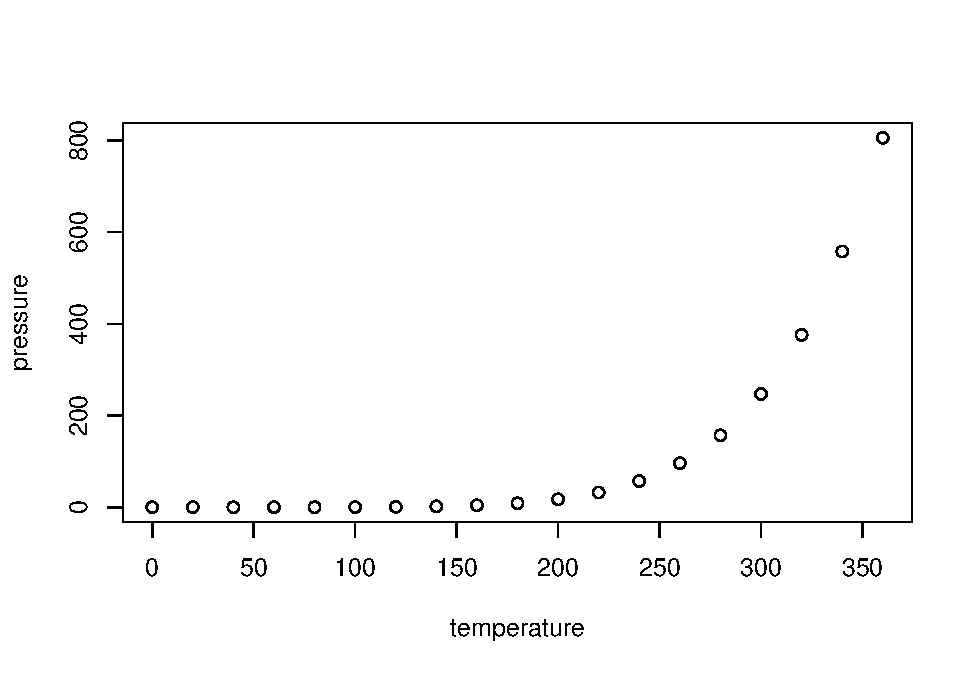
\includegraphics{_main_files/figure-latex/pressure-1.pdf}

Note that the \texttt{echo\ =\ FALSE} parameter was added to the code chunk to prevent printing of the R code that generated the plot.

  \bibliography{book.bib,packages.bib}

\end{document}
